\chapter{Methods}
\label{chapter:methods}

\section{Qt Developer Days 2011 Conference Schedule Application}
\label{section:devdays}

The Qt Developer
Days\footnote{\url{http://qt.nokia.com/qtdevdays2011/}} is a
conference for developers using the Qt cross-platform application and
\abbr{UI} framework\footnote{\url{http://qt.nokia.com/}}. We created a
mobile web application with contextual and personalized session
information and daily schedule for the conference.

\subsection{Requirements}



\subsection{Application Architecture}

\begin{figure}[ht]
  \begin{center}
    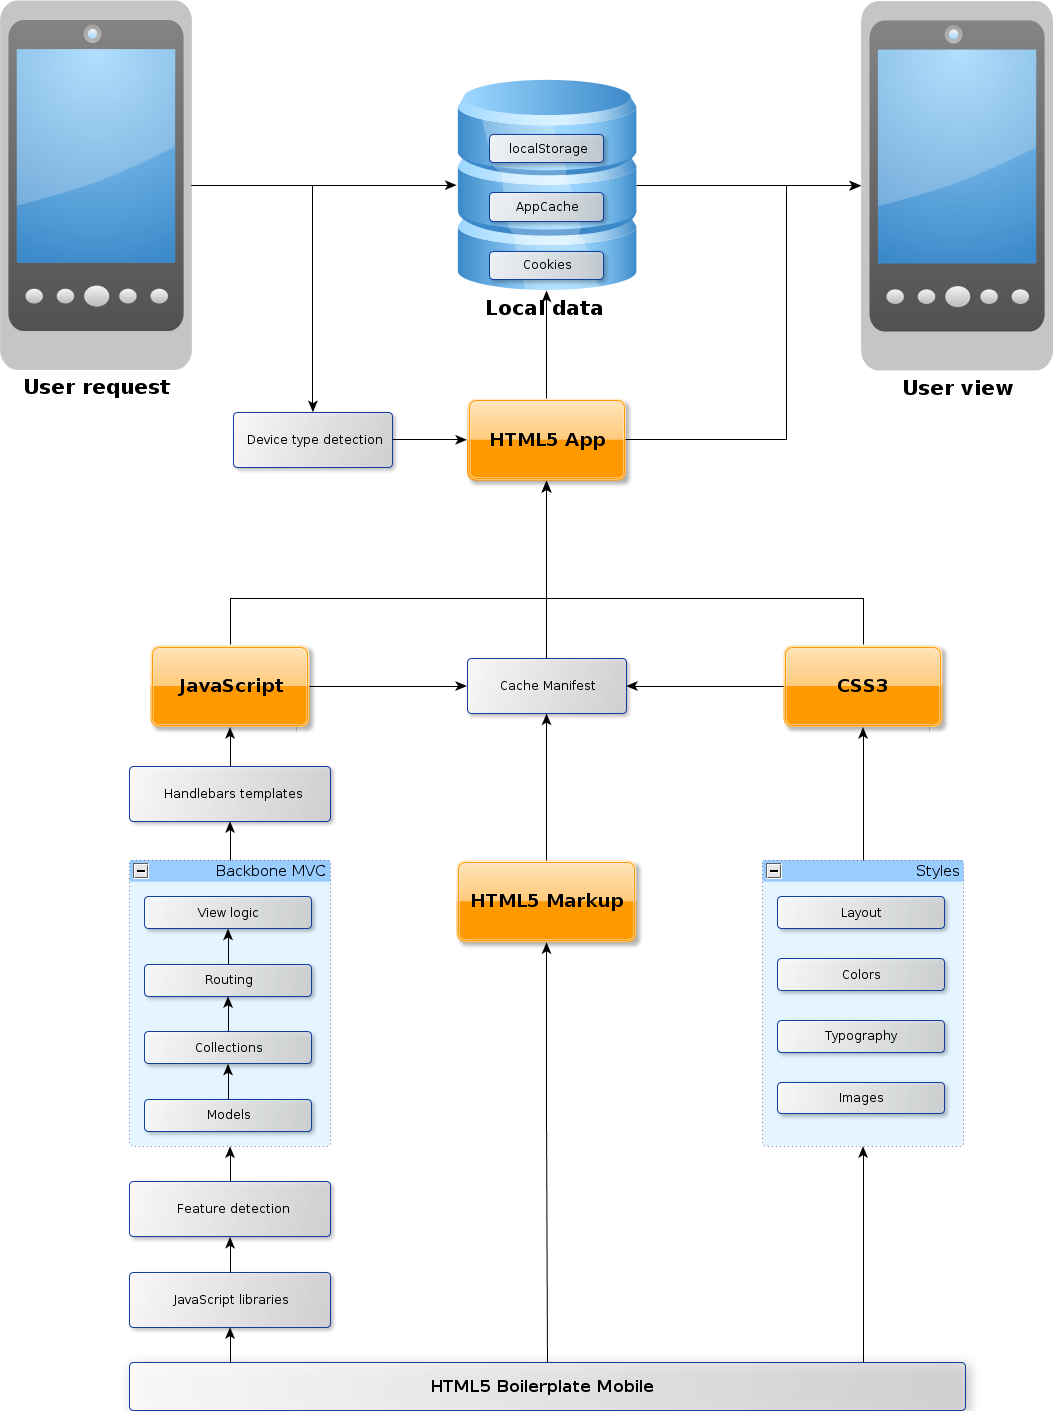
\includegraphics[width=\textwidth]{images/devdays.png}
    \caption{Conference schedule application architecture.}
    \label{figure:devdays.png}
  \end{center}
\end{figure}

The conference
schedule\footnote{\url{http://m.qtdevdays2011.qt.nokia.com/}} is a
single-page application \citationneeded with a lightweight backend
written in Python using the Django Web
Framework\footnote{\url{https://www.djangoproject.com/}}.

The backend provides the static assets (JavaScript, \abbr{CSS},
images, etc.) and an \abbr{API} for persisting session feedback to a
MySQL\footnote{\url{http://www.mysql.com/}} relational database. It
also generates the HTML5 AppCache \citationneeded offline cache
manifest file based on the categorized device type.

The frontend is a JavaScript application written using the
Backbone\footnote{\url{http://backbonejs.org/}} \abbr{MVC}
framework. Other used JavaScript libraries include
Underscore\footnote{\url{http://underscorejs.org/}} for data
manipulation, jQuery\footnote{\url{http://jquery.com/}} for \abbr{DOM}
API abstraction, Handlebars\footnote{\url{http://handlebarsjs.com/}}
for templating, and
Modernizr\footnote{\url{http://www.modernizr.com/}} for feature
detection. The HTML5 Mobile
Boilerplate\footnote{\url{http://html5boilerplate.com/mobile}} was
used as an initial markup structure for the application. The
architecture of is depicted in Figure~\ref{figure:devdays.png}.

Wireless networks can be unreliable in conference settings, so offline
support was also added using several different JavaScript techniques
and HTML5 APIs.

The application was designed for touch screens on various platforms
and screen sizes. The layout adjusts to the available space and
provides rich interactive components. Integration to social networking
services was also added as an additional functionality.

\fixme{add screenshots on different devices (at least phone and tablet}

\section{JSONCache JavaScript Library}
\label{section:jsoncache}

JSONCache is a lightweight JavaScript library for fetching \abbr{JSON}
data in unreliable networks. The library was designed especially to
handle unreliable mobile networks with connection problems and short
interruptions. The goal is to avoid networking as long as possible and
failing gracefully if the network connections are not stable.

JSONCache provides two main functionalities: data caching and
attempting to fetch the data multiple times.

The caching layer uses the client side localStorage \citationneeded
cache of \abbr{HTML5}. Data requests can be done using the JSONCache
\abbr{API} which always checks the local cache first before opening
any network connections. If the data is already in the cache, the
cached data is checked for validity and if the data has not been
expired, it is returned immediately. If the data is not in the cache
or it has been expired, a new network request is made and the received
data is cached and returned. The expiration time of a data item can be
configured in the library settings.

JSONCache also tries to fetch the data multiple times to handle small
interruptions in network connections. \fixme{add example and explain
  that it is very common}. If a data fetch fails, a new fetch is
issued after a timeout (defined in the configuration). On subsequent
attempts the timeout is increased, and after a defined number of
attempts the fetch error is issued.

Figure~\ref{figure:jsoncache-demo.png} shows an interactive demo of
the JSONCache library. The
demo\footnote{\url{http://kpuputti.github.com/JSONCache/demo/index.html}}
simulates the caching and fetching functionality of the library by
simulating a unreliable network based on the configuration.

\begin{figure}[ht]
  \begin{center}
    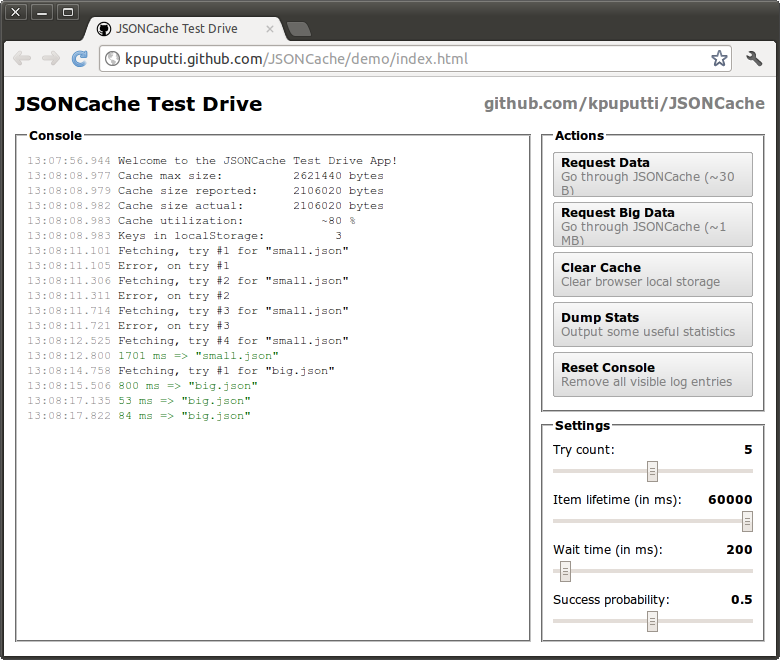
\includegraphics[width=\textwidth]{images/jsoncache-demo.png}
    \caption{Interactive JSONCache demo.}
    \label{figure:jsoncache-demo.png}
  \end{center}
\end{figure}
